\documentclass{article}

% Language setting
\usepackage[italian]{babel}

% Set page size and margins
\usepackage[a4paper,top=2cm,bottom=2cm,left=3cm,right=3cm,marginparwidth=1.75cm]{geometry}

% Useful packages
\usepackage{amsmath}
\usepackage{graphicx}
\usepackage{float}
\usepackage{marginnote}
\usepackage{enumitem}
\usepackage{array}
\usepackage{longtable}
\usepackage{booktabs}
\usepackage{xcolor}
\usepackage{listings}
\usepackage[colorlinks=true, allcolors=blue]{hyperref}

% Colonne a larghezza fissa con a-capo automatico
\newcolumntype{L}[1]{>{\raggedright\arraybackslash}p{#1}}
\newcommand{\code}[1]{\texttt{\small #1}}

% Stile per il listing YAML dell'OpenAPI
\definecolor{yamlkey}{rgb}{0.0,0.3,0.6}
\definecolor{yamlstr}{rgb}{0.6,0.2,0.0}
\definecolor{yamlcom}{rgb}{0.4,0.4,0.4}
\lstdefinelanguage{yaml}{
  keywords={true,false,null},
  sensitive=false,
  comment=[l]{\#},
  morestring=[b]',
  morestring=[b]"
}
\lstset{
  language=yaml,
  basicstyle=\ttfamily\tiny,
  keywordstyle=\color{yamlstr},
  stringstyle=\color{yamlstr},
  commentstyle=\color{yamlcom}\itshape,
  breaklines=true,
  breakatwhitespace=true,
  columns=fullflexible,
  showstringspaces=false,
  numbers=left,
  numberstyle=\ttfamily\tiny\color{yamlcom},
  numbersep=6pt,
  frame=lines,
  framexleftmargin=4pt,
  tabsize=2,
  extendedchars=true,
  literate=%
    {à}{{\`a}}1 {è}{{\`e}}1 {é}{{\'e}}1 {ì}{{\`i}}1 {ò}{{\`o}}1 {ù}{{\`u}}1
    {È}{{\`E}}1 {—}{{---}}1
}

\title{Deliverable 2 v1.0 \\ \large Documento di Sviluppo --- IoSonoTrento}
\author{Riccardo Sandru, Ernesto Beltrami, Tawfiq Songne}
\date{\today}

\begin{document}
\maketitle

\begin{abstract}
	Il presente documento riporta le informazioni necessarie allo sviluppo dell'applicazione
	\textit{IoSonoTrento}, la piattaforma di partecipazione civica per la città di Trento.
	Partendo dalla presentazione delle Web API del servizio, si prosegue con l'organizzazione
	del codice, la strategia di branching, le dipendenze, il modello dati e il testing.
	Infine, una sezione è dedicata al front-end e una agli aspetti di deployment.
\end{abstract}

\setcounter{tocdepth}{2}
\tableofcontents
\newpage

% ======================================================================
\section{Web API}
% ======================================================================

Le API sono state documentate secondo le specifiche \textbf{OpenAPI 3.0} e la documentazione
è consultabile in modo interattivo tramite \textbf{Swagger UI}, esposta dall'applicazione
all'indirizzo \code{http://localhost:8000/docs} quando il backend è in esecuzione.
La specifica non è mantenuta come file statico, bensì generata a runtime con
\code{swagger-jsdoc} a partire dalle annotazioni contenute nei file
\code{backend/src/swagger/*.paths.js} (uno per dominio applicativo) e assemblata in
\code{backend/src/config/swagger.js}.

\subsection*{Note sulle scelte di design delle API}
\begin{itemize}
	\item \textbf{Autenticazione a due ruoli}: tutte le rotte protette richiedono un token
	JWT \textit{Bearer}. Il ruolo (\code{operatore} oppure \code{cittadino}) è codificato nel
	token e usato per il \textit{role gating} (middleware \code{restrictTo}).
	\item \textbf{Risorsa Consultazione polimorfa}: una \code{Votazione} e un \code{Sondaggio}
	condividono lo stesso modello base (\code{Consultazione}) ma sono esposte tramite due
	gruppi di rotte distinti (\code{/votazioni} e \code{/sondaggi}) per chiarezza semantica.
	\item \textbf{Separazione lettura/scrittura per ruolo}: gli operatori gestiscono il ciclo
	di vita dei contenuti (creazione, pubblicazione, archiviazione, moderazione), mentre i
	cittadini dispongono di rotte dedicate alla consultazione e all'espressione del voto
	(prefisso \code{/cittadino/vote/...}).
	\item \textbf{Validazione degli identificatori}: le rotte con parametro \code{/:id} sono
	protette dal middleware \code{validateObjectId}, che restituisce \code{400} per ObjectId
	non validi prima di interrogare il database.
\end{itemize}

\subsection*{Riepilogo degli endpoint}
La seguente tabella riassume gli endpoint esposti, raggruppati per dominio. La specifica
completa OpenAPI è riportata in \hyperref[app:openapi]{Appendice A}.

\renewcommand{\arraystretch}{1.2}
\begin{longtable}{L{2.6cm} L{6.2cm} L{4.4cm}}
	\toprule
	\textbf{Metodo} & \textbf{Endpoint} & \textbf{Ruolo} \\
	\midrule
	\endhead
	\multicolumn{3}{l}{\textit{Autenticazione}} \\
	GET    & \code{/auth/google} & pubblico \\
	GET    & \code{/auth/google/callback} & pubblico \\
	POST   & \code{/auth/complete-profile} & cittadino (1° accesso) \\
	\midrule
	\multicolumn{3}{l}{\textit{Operatore}} \\
	POST   & \code{/operatore/login} & pubblico \\
	POST   & \code{/operatore/register} & operatore \\
	GET    & \code{/operatore/profile} & operatore \\
	PATCH  & \code{/operatore/me/password} & operatore \\
	PATCH  & \code{/operatore/\{id\}/promote} & operatore root \\
	\midrule
	\multicolumn{3}{l}{\textit{Cittadino}} \\
	GET    & \code{/cittadino/profile} & cittadino \\
	POST   & \code{/cittadino/logout} & cittadino \\
	POST   & \code{/cittadino/vote/votazione} & cittadino \\
	POST   & \code{/cittadino/vote/sondaggio} & cittadino \\
	POST   & \code{/cittadino/vote/iniziativa} & cittadino \\
	DELETE & \code{/cittadino/vote/iniziativa/\{id\}} & cittadino \\
	\midrule
	\multicolumn{3}{l}{\textit{Votazioni}} \\
	GET / POST & \code{/votazioni} & lettura / operatore \\
	GET        & \code{/votazioni/cittadino} & cittadino \\
	GET / PATCH / DELETE & \code{/votazioni/\{id\}} & lettura / operatore \\
	PATCH      & \code{/votazioni/\{id\}/publish} & operatore \\
	PATCH      & \code{/votazioni/\{id\}/archive} & operatore \\
	GET        & \code{/votazioni/\{id\}/riepilogo} & autenticato \\
	\midrule
	\multicolumn{3}{l}{\textit{Sondaggi}} \\
	GET / POST & \code{/sondaggi} & lettura / operatore \\
	GET        & \code{/sondaggi/cittadino} & cittadino \\
	GET / PATCH / DELETE & \code{/sondaggi/\{id\}} & lettura / operatore \\
	PATCH      & \code{/sondaggi/\{id\}/publish} & operatore \\
	PATCH      & \code{/sondaggi/\{id\}/archive} & operatore \\
	GET        & \code{/sondaggi/\{id\}/riepilogo} & autenticato \\
	\midrule
	\multicolumn{3}{l}{\textit{Iniziative}} \\
	GET / POST & \code{/iniziative} & cittadino / lettura \\
	POST       & \code{/iniziative/ricerca} & autenticato \\
	GET / PATCH / DELETE & \code{/iniziative/\{id\}} & autenticato \\
	PATCH      & \code{/iniziative/\{id\}/modera} & operatore \\
	\midrule
	\multicolumn{3}{l}{\textit{Categorie e Notifiche}} \\
	GET / POST & \code{/categorie} & lettura / operatore \\
	GET / PATCH / DELETE & \code{/categorie/\{id\}} & lettura / operatore \\
	GET        & \code{/notifiche} & cittadino \\
	PATCH      & \code{/notifiche/leggi-tutte} & cittadino \\
	PATCH      & \code{/notifiche/\{id\}/letta} & cittadino \\
	\bottomrule
\end{longtable}

% ======================================================================
\section{Implementation}
% ======================================================================

L'applicazione è composta da un \textbf{backend} realizzato in NodeJS con il framework
Express e da un \textbf{frontend} sviluppato in React. La persistenza dei dati è affidata a
MongoDB, interrogato tramite l'ODM Mongoose. Lo stack tecnologico è stato scelto sulla base
del materiale fornito nel corso e delle conoscenze pregresse del gruppo, privilegiando un
ecosistema JavaScript omogeneo dal database al client.

\subsection{Repository Organization}

Il codice del progetto è ospitato su GitHub
(\url{https://github.com/ErnestoBeltrami/Ingegneria_Software}). La struttura è la seguente:

\begin{itemize}[leftmargin=2cm]
	\item[\code{deliverable\_1/}] documentazione (analisi, requisiti, use case)
	\item[\code{deliverable\_2/}] codice dell'applicazione
	\begin{itemize}[leftmargin=1.5cm]
		\item[\code{backend/}] codice del server
		\begin{itemize}[leftmargin=1.5cm]
			\item[\code{src/routes/}] definizione degli endpoint Express
			\item[\code{src/controllers/}] logica applicativa dei vari domini
			\item[\code{src/models/}] schemi dati Mongoose
			\item[\code{src/middleware/}] autenticazione e autorizzazione
			\item[\code{src/swagger/}] definizioni OpenAPI per dominio
			\item[\code{src/config/}] configurazione (DB, Swagger, Passport)
			\item[\code{src/utils/}] scheduler e script di \textit{seed}
			\item[\code{tests/}] test unitari Jest e file \code{.rest} manuali
		\end{itemize}
		\item[\code{frontend/}] applicazione React (Vite)
		\item[\code{docs/}] documentazione e specifica OpenAPI esportata
		\item[\code{package.json}] configurazione del progetto npm
		\item[\code{.env}] variabili d'ambiente (non versionato)
	\end{itemize}
\end{itemize}

\subsection{Branching strategy e organizzazione del lavoro}

Lo sviluppo ha visto una collaborazione attiva tra i membri del gruppo. A livello di
repository abbiamo adottato una strategia di branching ispirata a \textbf{GitFlow}: il branch
\code{main} contiene le versioni stabili, mentre ogni nuova funzionalità o correzione è stata
sviluppata su un branch dedicato, derivato da \code{main} e reintegrato tramite
\textit{Pull Request} con revisione tra pari prima del merge.

I branch seguono una convenzione di prefisso che ne esplicita la natura:
\begin{itemize}
	\item \code{feature/...} e \code{feat/...} --- nuove funzionalità (es.\ \code{feature/votazione},
	\code{feature/bacheca}, \code{feature/dashboard}, \code{feat/moderazione-bacheca},
	\code{feat/paginazione-liste});
	\item \code{frontend/...} --- sviluppo delle interfacce (es.\ \code{frontend/login},
	\code{frontend/dashboard}, \code{frontend/riepilogoVotazione});
	\item \code{fix/...} --- correzioni di bug (es.\ \code{fix/modifica-precompila-form},
	\code{fix/no-error-leak-in-responses}, \code{fix/sondaggio-get-by-id-cittadino}).
\end{itemize}

Il lavoro è stato suddiviso tra i membri del gruppo per aree funzionali (gestione
votazioni/sondaggi, bacheca delle iniziative, autenticazione, dashboard e front-end).
Eventuali sbilanciamenti nel numero di commit per autore sono dovuti a differenze nella
granularità dei commit (molti commit piccoli rispetto a pochi commit più consistenti) e non
riflettono necessariamente il volume di lavoro svolto.

\subsection{Dependencies}

Il backend si basa sui seguenti moduli principali di produzione:

\renewcommand{\arraystretch}{1.15}
\begin{longtable}{L{4cm} L{9cm}}
	\toprule
	\textbf{Modulo} & \textbf{Utilizzo} \\
	\midrule
	\endhead
	express              & Framework web per il backend (v5) \\
	mongoose             & ODM per interfacciarsi con MongoDB \\
	passport / passport-google-oauth20 & Autenticazione dei cittadini tramite Google OAuth 2.0 \\
	jsonwebtoken         & Generazione e verifica dei token JWT \\
	bcryptjs             & Hashing delle password degli operatori \\
	express-session      & Gestione della sessione durante il flusso OAuth \\
	express-rate-limit   & Limitazione del numero di richieste (anti-abuso) \\
	node-cron            & Scheduler per le transizioni di stato delle consultazioni \\
	pino / pino-http     & Logging strutturato delle richieste \\
	swagger-jsdoc / swagger-ui-express & Generazione ed esposizione della documentazione OpenAPI \\
	dotenv               & Caricamento delle variabili d'ambiente da file \code{.env} \\
	\bottomrule
\end{longtable}

\noindent E le seguenti dipendenze di sviluppo:

\begin{longtable}{L{4cm} L{9cm}}
	\toprule
	\textbf{Modulo} & \textbf{Utilizzo} \\
	\midrule
	jest          & Framework per i test unitari (modalità ESM) \\
	supertest     & Test di integrazione sugli endpoint Express \\
	nodemon       & Auto-reload del server in fase di sviluppo \\
	concurrently  & Avvio simultaneo di backend e frontend \\
	pino-pretty   & Formattazione leggibile dei log in sviluppo \\
	\bottomrule
\end{longtable}

\noindent Il frontend utilizza \textbf{React 18} con \textbf{Vite} come build tool e
\textbf{TailwindCSS} (con DaisyUI) per lo styling. Per la navigazione è impiegato
\code{react-router-dom}, per le animazioni \code{framer-motion}, per le icone
\code{lucide-react} e per i grafici dei riepiloghi \code{recharts}.

\subsection{Database}

La persistenza è gestita su MongoDB tramite Mongoose. Il modello dati è organizzato nelle
seguenti collezioni principali:

\renewcommand{\arraystretch}{1.15}
\begin{longtable}{L{4cm} L{9cm}}
	\toprule
	\textbf{Modello} & \textbf{Descrizione dei campi principali} \\
	\midrule
	\endhead
	Operatore            & \code{username}, \code{password} (bcrypt), flag \code{isRoot} \\
	Cittadino            & \code{email}, \code{ID\_univoco\_esterno} (Google ID),
	                       \code{profiloCompleto}, \code{loggedIn} \\
	Consultazione        & \code{tipo} (\code{votazione}/\code{sondaggio}),
	                       \code{stato} (\code{bozza}$\to$\code{attivo}$\to$\code{concluso}$\to$\code{archiviato}),
	                       \code{titolo}, \code{descrizione}, date e \code{creatoDa} \\
	Domanda              & \code{titolo}, \code{opzioni[]},
	                       \code{tipo} (\code{risposta\_singola}/\code{risposta\_multipla}) \\
	Iniziativa           & \code{titolo}, \code{descrizione}, \code{ID\_cittadino},
	                       \code{ID\_categoria}, \code{stato}, \code{motivazione\_moderazione} \\
	VotoIniziativa       & Relazione tra Cittadino e Iniziativa \\
	RispostaConsultazione& Risposta di un cittadino a una Consultazione \\
	CategoriaIniziativa  & \code{nome} della categoria tematica \\
	Notifica             & \code{ID\_destinatario}, \code{tipo}, \code{messaggio},
	                       \code{ID\_iniziativa}, flag \code{letta} \\
	\bottomrule
\end{longtable}

Il vincolo chiave del dominio riguarda la \code{Consultazione}: una \code{votazione} è
associata a una singola domanda (\code{ID\_domanda}), mentre un \code{sondaggio} è associato a
un array di domande (\code{ID\_domande[]}). I due casi sono mutuamente esclusivi e tale
vincolo è imposto da validatori Mongoose. Le transizioni di stato delle consultazioni
(\code{bozza}$\to$\code{attivo}$\to$\code{concluso}) sono gestite automaticamente da uno
scheduler basato su \code{node-cron} (\code{utils/scheduleConsultazioni.js}), eseguito
all'avvio e successivamente con cadenza oraria. Al primo avvio lo script \code{seedRoot.js}
crea automaticamente un account operatore \code{isRoot} con credenziali iniziali note.

\subsection{Testing}

Il codice del backend è corredato di una test-suite che ne verifica il corretto
funzionamento. I test unitari sono implementati con \textbf{Jest} (in modalità ESM) e sono
organizzati nella cartella \code{backend/tests/unit/}, con un file per ciascun controller
principale. Complessivamente sono definiti \textbf{44 casi di test} così distribuiti:

\begin{itemize}
	\item \code{consultazione.controller.test.js} --- 18 test;
	\item \code{sondaggio.controller.test.js} --- 11 test;
	\item \code{votazione.controller.test.js} --- 8 test;
	\item \code{iniziativa.controller.test.js} --- 4 test;
	\item \code{seedRoot.test.js} --- 3 test.
\end{itemize}

L'esecuzione avviene tramite \code{npm test} (oppure \code{npm run test:coverage} per il
report di copertura). Oltre ai test automatici, sono presenti file di test manuali degli
endpoint in formato \code{.rest} (\code{backend/tests/rest/}), uno per dominio applicativo,
eseguibili con gli script \code{npm run test:api:*}. Il relativo runner gestisce
automaticamente il login JWT e la risoluzione delle variabili dinamiche
(es.\ \code{\{\{TOKEN\_OPERATORE\}\}}, \code{\{\{VOTAZIONE\_ID\}\}}) tra richieste successive.

A titolo di esempio, la seguente tabella riporta alcuni casi di test relativi alla creazione
di un account operatore:

\renewcommand{\arraystretch}{1.3}
\begin{longtable}{L{0.8cm} L{3.4cm} L{3cm} L{4.5cm}}
	\toprule
	\textbf{N.} & \textbf{Descrizione} & \textbf{Dati di test} & \textbf{Risultato atteso} \\
	\midrule
	\endhead
	1 & Creazione account corretta & username non vuoto, password conforme alle policy &
	L'account viene creato; il sistema risponde con esito positivo \\
	1.1 & Creazione con username già esistente & username già presente nel sistema &
	Errore \textit{user exists}, l'account non viene creato \\
	2 & Creazione senza username & username vuoto &
	Errore \textit{empty user}, l'account non viene creato \\
	3 & Password non conforme & password che viola le policy di sicurezza &
	Errore di validazione, l'account non viene creato \\
	\bottomrule
\end{longtable}

% ======================================================================
\section{FrontEnd}
% ======================================================================

Il front-end è una \textit{Single Page Application} realizzata in React e servita da Vite.
Fornisce le funzionalità di visualizzazione, inserimento e gestione dei dati
dell'applicazione, con due aree distinte in base al ruolo dell'utente autenticato.

\paragraph{Area pubblica e autenticazione.}
La \code{LandingPage} presenta il progetto e instrada l'utente verso il login. I cittadini
accedono tramite Google OAuth (\code{LoginPage}, \code{AuthCallbackPage}) e, al primo accesso,
completano il profilo (\code{CompletaProfiloPage}). Gli operatori accedono con
username e password.

\paragraph{Area cittadino.}
Comprende la dashboard con le consultazioni attive
(\code{DashboardCittadinePage}), le pagine di voto per votazioni e sondaggi
(\code{Votazione}, \code{VotaSondaggio}), i riepiloghi dei risultati con grafici
(\code{RiepilogoVotazione}, \code{RiepilogoSondaggio}), la bacheca delle iniziative con
creazione e voto (\code{BachecaPage}, \code{CreaIniziativaPage}), l'archivio delle
consultazioni concluse (\code{ArchivioPage}) e il profilo personale.

\paragraph{Area operatore.}
Comprende la dashboard amministrativa (\code{DashboardOperatorePage}), la creazione e modifica
di votazioni e sondaggi (\code{CreaVotazionePage}, \code{ModificaVotazionePage},
\code{CreaSondaggioPage}, \code{ModificaSondaggioPage}), la gestione del ciclo di vita delle
consultazioni (\code{GestioneVotazioniPage}, \code{GestioneSondaggiPage}), la moderazione
della bacheca (\code{ModerazioneBachecaPage}) e i riepiloghi di dettaglio dei risultati.

\bigskip
\noindent Di seguito alcune schermate rappresentative dell'applicazione.

\begin{figure}[H]
	\centering
	
\includegraphics[width=0.9\textwidth]{images/landingPage.png}
	\caption{Landing page dell'applicazione IoSonoTrento.}
\end{figure}

\begin{figure}[H]
	\centering
	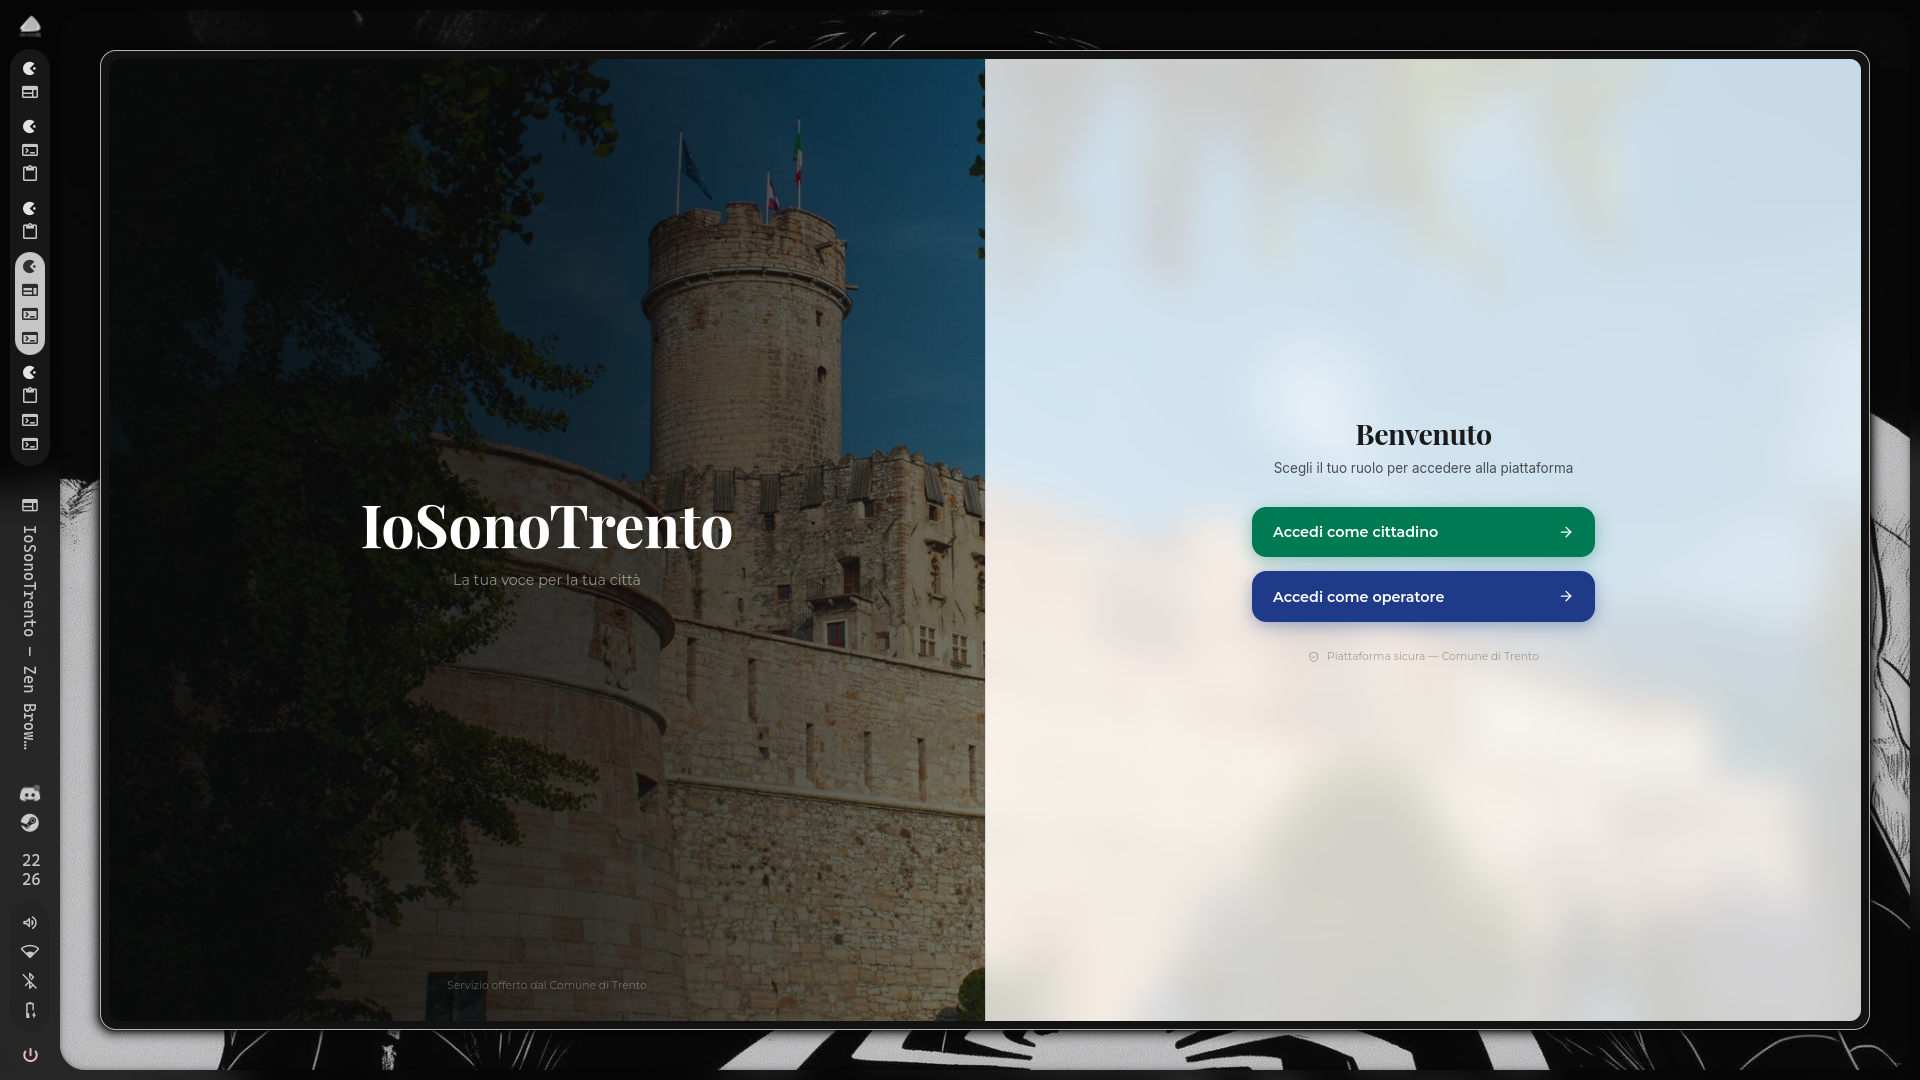
\includegraphics[width=0.9\textwidth]{images/loginPage.png}
	\caption{Pagina di login.}
\end{figure}

\begin{figure}[H]
	\centering
	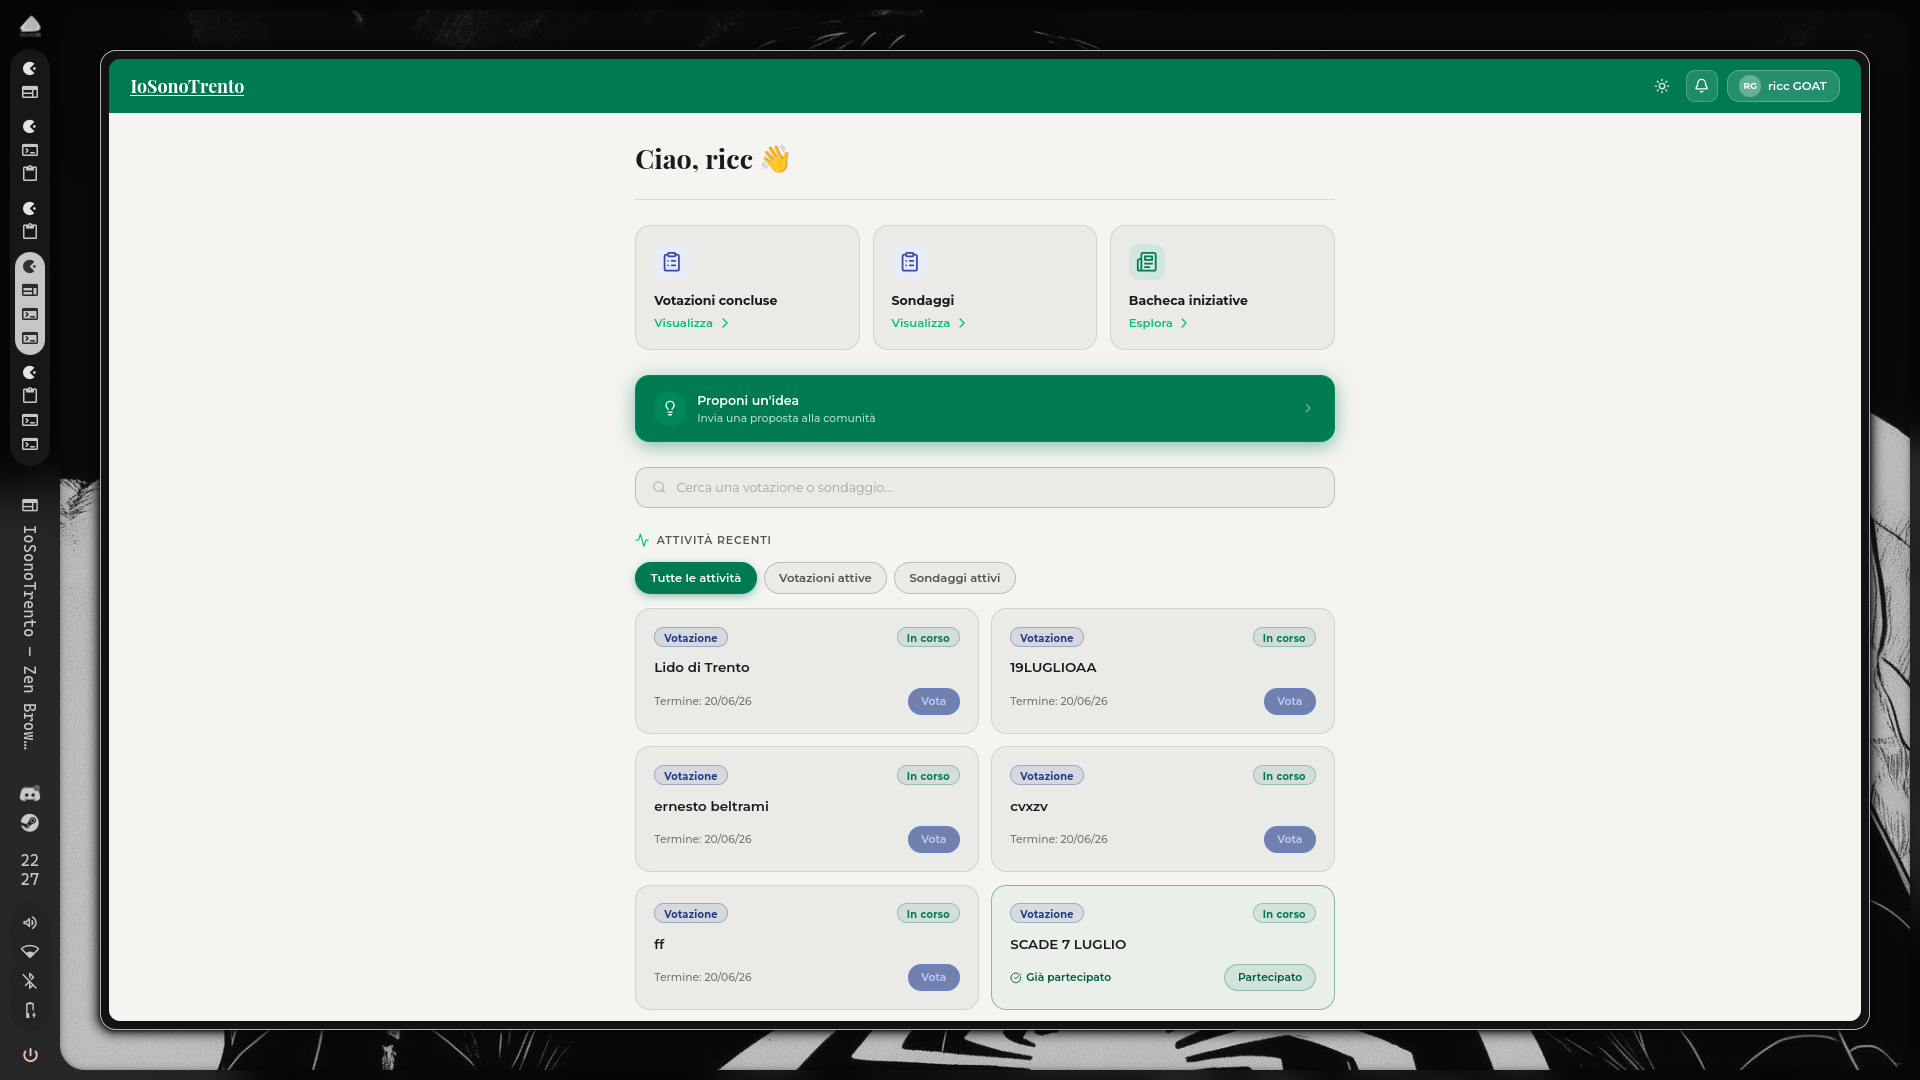
\includegraphics[width=0.9\textwidth]{images/dashboardCittadino.png}
	\caption{Dashboard del cittadino con le consultazioni attive.}
\end{figure}

\begin{figure}[H]
	\centering
	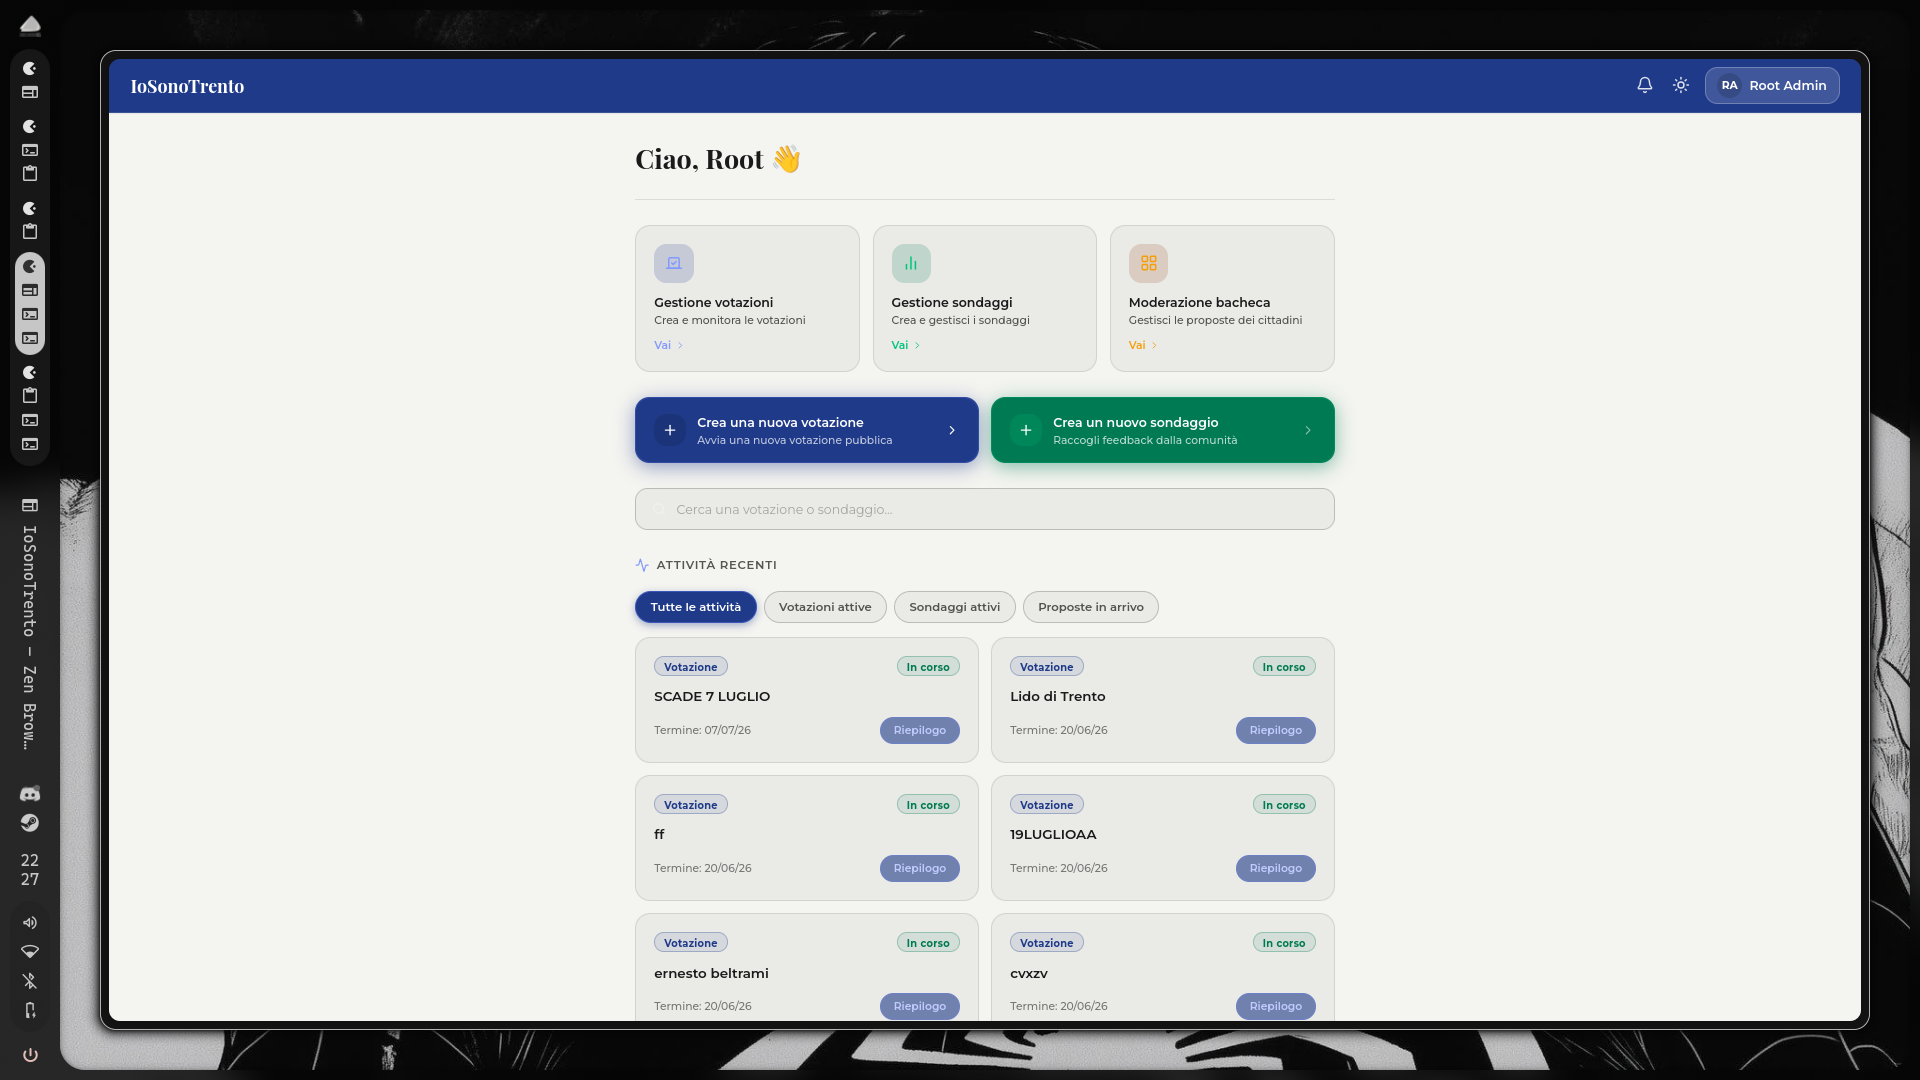
\includegraphics[width=0.9\textwidth]{images/dashboardOperatore.png}
	\caption{Dashboard dell'operatore per la gestione dei contenuti.}
\end{figure}

% ======================================================================
\section{Deployment}
% ======================================================================

Allo stato attuale l'applicazione viene eseguita in ambiente locale di sviluppo. Per l'avvio
è necessario disporre di un'istanza MongoDB attiva e di un file \code{.env} configurato (porta,
segreti di sessione e JWT, URI del database e, opzionalmente, le credenziali Google OAuth).

\paragraph{Avvio in locale.}
Dalla cartella \code{deliverable\_2/}:
\begin{itemize}
	\item \code{npm install} --- installazione delle dipendenze del backend;
	\item \code{npm run dev} --- avvio del solo backend con auto-reload;
	\item \code{npm run dev:all} --- avvio simultaneo di backend e frontend (\code{concurrently}).
\end{itemize}
Verifiche rapide: \textit{health check} su \code{http://localhost:8000/health} e
documentazione API su \code{http://localhost:8000/docs}.

\paragraph{Deployment futuro \textnormal{(da completare)}.}
È prevista la pubblicazione dell'applicazione su una piattaforma di hosting cloud, con
configurazione di una pipeline CI/CD basata su GitHub Actions che esegua automaticamente il
deploy del branch \code{main} al superamento dei test.

\begin{itemize}
	\item Backend deployato all'indirizzo: \texttt{<<link backend>>}
	\item Frontend deployato all'indirizzo: \texttt{<<link frontend>>}
	\item Account dimostrativi di accesso: \texttt{<<credenziali demo>>}
	\item Riferimento per problemi di deploy: \texttt{<<contatto/mail>>}
\end{itemize}

\newpage
% ======================================================================
\appendix
\section{Specifica OpenAPI completa}
\label{app:openapi}
% ======================================================================

Di seguito è riportata per esteso la specifica OpenAPI 3.0 dell'applicazione, generata a
partire dalle annotazioni del codice ed esportata nel file \code{docs/openapi.yaml}.

\lstinputlisting{openapi.yaml}

\end{document}
